% Options for packages loaded elsewhere
\PassOptionsToPackage{unicode}{hyperref}
\PassOptionsToPackage{hyphens}{url}
%
\documentclass[
]{article}
\usepackage{lmodern}
\usepackage{amssymb,amsmath}
\usepackage{ifxetex,ifluatex}
\ifnum 0\ifxetex 1\fi\ifluatex 1\fi=0 % if pdftex
  \usepackage[T1]{fontenc}
  \usepackage[utf8]{inputenc}
  \usepackage{textcomp} % provide euro and other symbols
\else % if luatex or xetex
  \usepackage{unicode-math}
  \defaultfontfeatures{Scale=MatchLowercase}
  \defaultfontfeatures[\rmfamily]{Ligatures=TeX,Scale=1}
\fi
% Use upquote if available, for straight quotes in verbatim environments
\IfFileExists{upquote.sty}{\usepackage{upquote}}{}
\IfFileExists{microtype.sty}{% use microtype if available
  \usepackage[]{microtype}
  \UseMicrotypeSet[protrusion]{basicmath} % disable protrusion for tt fonts
}{}
\makeatletter
\@ifundefined{KOMAClassName}{% if non-KOMA class
  \IfFileExists{parskip.sty}{%
    \usepackage{parskip}
  }{% else
    \setlength{\parindent}{0pt}
    \setlength{\parskip}{6pt plus 2pt minus 1pt}}
}{% if KOMA class
  \KOMAoptions{parskip=half}}
\makeatother
\usepackage{xcolor}
\IfFileExists{xurl.sty}{\usepackage{xurl}}{} % add URL line breaks if available
\IfFileExists{bookmark.sty}{\usepackage{bookmark}}{\usepackage{hyperref}}
\hypersetup{
  hidelinks,
  pdfcreator={LaTeX via pandoc}}
\urlstyle{same} % disable monospaced font for URLs
\usepackage{color}
\usepackage{fancyvrb}
\newcommand{\VerbBar}{|}
\newcommand{\VERB}{\Verb[commandchars=\\\{\}]}
\DefineVerbatimEnvironment{Highlighting}{Verbatim}{commandchars=\\\{\}}
% Add ',fontsize=\small' for more characters per line
\newenvironment{Shaded}{}{}
\newcommand{\AlertTok}[1]{\textcolor[rgb]{1.00,0.00,0.00}{\textbf{#1}}}
\newcommand{\AnnotationTok}[1]{\textcolor[rgb]{0.38,0.63,0.69}{\textbf{\textit{#1}}}}
\newcommand{\AttributeTok}[1]{\textcolor[rgb]{0.49,0.56,0.16}{#1}}
\newcommand{\BaseNTok}[1]{\textcolor[rgb]{0.25,0.63,0.44}{#1}}
\newcommand{\BuiltInTok}[1]{#1}
\newcommand{\CharTok}[1]{\textcolor[rgb]{0.25,0.44,0.63}{#1}}
\newcommand{\CommentTok}[1]{\textcolor[rgb]{0.38,0.63,0.69}{\textit{#1}}}
\newcommand{\CommentVarTok}[1]{\textcolor[rgb]{0.38,0.63,0.69}{\textbf{\textit{#1}}}}
\newcommand{\ConstantTok}[1]{\textcolor[rgb]{0.53,0.00,0.00}{#1}}
\newcommand{\ControlFlowTok}[1]{\textcolor[rgb]{0.00,0.44,0.13}{\textbf{#1}}}
\newcommand{\DataTypeTok}[1]{\textcolor[rgb]{0.56,0.13,0.00}{#1}}
\newcommand{\DecValTok}[1]{\textcolor[rgb]{0.25,0.63,0.44}{#1}}
\newcommand{\DocumentationTok}[1]{\textcolor[rgb]{0.73,0.13,0.13}{\textit{#1}}}
\newcommand{\ErrorTok}[1]{\textcolor[rgb]{1.00,0.00,0.00}{\textbf{#1}}}
\newcommand{\ExtensionTok}[1]{#1}
\newcommand{\FloatTok}[1]{\textcolor[rgb]{0.25,0.63,0.44}{#1}}
\newcommand{\FunctionTok}[1]{\textcolor[rgb]{0.02,0.16,0.49}{#1}}
\newcommand{\ImportTok}[1]{#1}
\newcommand{\InformationTok}[1]{\textcolor[rgb]{0.38,0.63,0.69}{\textbf{\textit{#1}}}}
\newcommand{\KeywordTok}[1]{\textcolor[rgb]{0.00,0.44,0.13}{\textbf{#1}}}
\newcommand{\NormalTok}[1]{#1}
\newcommand{\OperatorTok}[1]{\textcolor[rgb]{0.40,0.40,0.40}{#1}}
\newcommand{\OtherTok}[1]{\textcolor[rgb]{0.00,0.44,0.13}{#1}}
\newcommand{\PreprocessorTok}[1]{\textcolor[rgb]{0.74,0.48,0.00}{#1}}
\newcommand{\RegionMarkerTok}[1]{#1}
\newcommand{\SpecialCharTok}[1]{\textcolor[rgb]{0.25,0.44,0.63}{#1}}
\newcommand{\SpecialStringTok}[1]{\textcolor[rgb]{0.73,0.40,0.53}{#1}}
\newcommand{\StringTok}[1]{\textcolor[rgb]{0.25,0.44,0.63}{#1}}
\newcommand{\VariableTok}[1]{\textcolor[rgb]{0.10,0.09,0.49}{#1}}
\newcommand{\VerbatimStringTok}[1]{\textcolor[rgb]{0.25,0.44,0.63}{#1}}
\newcommand{\WarningTok}[1]{\textcolor[rgb]{0.38,0.63,0.69}{\textbf{\textit{#1}}}}
\usepackage{longtable,booktabs}
% Correct order of tables after \paragraph or \subparagraph
\usepackage{etoolbox}
\makeatletter
\patchcmd\longtable{\par}{\if@noskipsec\mbox{}\fi\par}{}{}
\makeatother
% Allow footnotes in longtable head/foot
\IfFileExists{footnotehyper.sty}{\usepackage{footnotehyper}}{\usepackage{footnote}}
\makesavenoteenv{longtable}
\usepackage{graphicx}
\makeatletter
\def\maxwidth{\ifdim\Gin@nat@width>\linewidth\linewidth\else\Gin@nat@width\fi}
\def\maxheight{\ifdim\Gin@nat@height>\textheight\textheight\else\Gin@nat@height\fi}
\makeatother
% Scale images if necessary, so that they will not overflow the page
% margins by default, and it is still possible to overwrite the defaults
% using explicit options in \includegraphics[width, height, ...]{}
\setkeys{Gin}{width=\maxwidth,height=\maxheight,keepaspectratio}
% Set default figure placement to htbp
\makeatletter
\def\fps@figure{htbp}
\makeatother
\setlength{\emergencystretch}{3em} % prevent overfull lines
\providecommand{\tightlist}{%
  \setlength{\itemsep}{0pt}\setlength{\parskip}{0pt}}
\setcounter{secnumdepth}{-\maxdimen} % remove section numbering

\author{}
\date{}

\begin{document}

\hypertarget{lecture-4-robust-analog-circuit-sizing-under-process-variations}{%
\section{Lecture 4: Robust Analog Circuit Sizing Under Process Variations}\label{lecture-4-robust-analog-circuit-sizing-under-process-variations}}

\hypertarget{luk036}{%
\subsection{@luk036}\label{luk036}}

2022-10-12

\hypertarget{keywords}{%
\subsection{🔑 Keywords}\label{keywords}}

\begin{itemize}
\tightlist
\item
  Analog circuit 模拟电路
\item
  Design for robustness 鲁棒性设计
\item
  Worst-case scenarios 最坏情景
\item
  Affine arithmetic 仿射运算
\item
  Convex programming 凸规划
\item
  Geometric programming 几何规划
\item
  Posynomial 正项式 (Positive + polynomial)
\item
  Ellipsoid method 椭球法
\end{itemize}

\hypertarget{overview}{%
\subsection{🗺️ Overview}\label{overview}}

\begin{itemize}
\item
  Challenges of 20nm Analog Design
\item
  Design for variability
\item
  Design for robustness
\item
  Analog circuit sizing problem formulation
\item
  Robust geometric programming
\item
  Affine arithmetic for worst case scenarios
\item
  Design examples
\end{itemize}

\hypertarget{introduction}{%
\subsection{📖 Introduction}\label{introduction}}

\begin{longtable}[]{@{}lll@{}}
\caption{Fab, process, mask, and design costs are much higher at 20nm (IBS,
May 2011)}\tabularnewline
\toprule
\begin{minipage}[b]{0.34\columnwidth}\raggedright
Costs\strut
\end{minipage} & \begin{minipage}[b]{0.26\columnwidth}\raggedright
28nm\strut
\end{minipage} & \begin{minipage}[b]{0.31\columnwidth}\raggedright
20nm\strut
\end{minipage}\tabularnewline
\midrule
\endfirsthead
\toprule
\begin{minipage}[b]{0.34\columnwidth}\raggedright
Costs\strut
\end{minipage} & \begin{minipage}[b]{0.26\columnwidth}\raggedright
28nm\strut
\end{minipage} & \begin{minipage}[b]{0.31\columnwidth}\raggedright
20nm\strut
\end{minipage}\tabularnewline
\midrule
\endhead
\begin{minipage}[t]{0.34\columnwidth}\raggedright
Fab Costs\strut
\end{minipage} & \begin{minipage}[t]{0.26\columnwidth}\raggedright
3B\strut
\end{minipage} & \begin{minipage}[t]{0.31\columnwidth}\raggedright
4B - 7B\strut
\end{minipage}\tabularnewline
\begin{minipage}[t]{0.34\columnwidth}\raggedright
Process R\&D\strut
\end{minipage} & \begin{minipage}[t]{0.26\columnwidth}\raggedright
1.2B\strut
\end{minipage} & \begin{minipage}[t]{0.31\columnwidth}\raggedright
2.1B - 3B\strut
\end{minipage}\tabularnewline
\begin{minipage}[t]{0.34\columnwidth}\raggedright
Mask Costs\strut
\end{minipage} & \begin{minipage}[t]{0.26\columnwidth}\raggedright
2M - 3M\strut
\end{minipage} & \begin{minipage}[t]{0.31\columnwidth}\raggedright
5M - 8M\strut
\end{minipage}\tabularnewline
\begin{minipage}[t]{0.34\columnwidth}\raggedright
Design Costs\strut
\end{minipage} & \begin{minipage}[t]{0.26\columnwidth}\raggedright
50M - 90M\strut
\end{minipage} & \begin{minipage}[t]{0.31\columnwidth}\raggedright
120M - 500M\strut
\end{minipage}\tabularnewline
\bottomrule
\end{longtable}

\hypertarget{challenges-at-20-nm}{%
\subsection{Challenges at 20 nm}\label{challenges-at-20-nm}}

\begin{itemize}
\item
  Double-patterning aware
\item
  Layout-dependent effects
\item
  New local interconnect layers
\item
  \textgreater5,000 design rules
\item
  Device variation and sensitivity
\item
  New type of transistor - FinFET
\end{itemize}

\hypertarget{double-patterning}{%
\subsection{Double Patterning}\label{double-patterning}}

\begin{figure}
\centering
\includegraphics{lec04.files/img001.png}
\caption{img}
\end{figure}

\hypertarget{overlay-error-mask-shift}{%
\subsection{Overlay Error (Mask Shift)}\label{overlay-error-mask-shift}}

\begin{itemize}
\item
  Parasitic matching becomes very challenging

  \begin{figure}
  \centering
  \includegraphics{lec04.files/img002.png}
  \caption{img}
  \end{figure}
\end{itemize}

\hypertarget{layout-dependent-effects}{%
\subsection{Layout-Dependent Effects}\label{layout-dependent-effects}}

\begin{longtable}[]{@{}lccc@{}}
\toprule
\begin{minipage}[b]{0.50\columnwidth}\raggedright
Layout-Dependent Effects\strut
\end{minipage} & \begin{minipage}[b]{0.12\columnwidth}\centering
\textgreater{} 40nm\strut
\end{minipage} & \begin{minipage}[b]{0.12\columnwidth}\centering
At 40nm\strut
\end{minipage} & \begin{minipage}[b]{0.14\columnwidth}\centering
\textgreater= 28nm\strut
\end{minipage}\tabularnewline
\midrule
\endhead
\begin{minipage}[t]{0.50\columnwidth}\raggedright
Well Proximity Effect (WPE)\strut
\end{minipage} & \begin{minipage}[t]{0.12\columnwidth}\centering
x\strut
\end{minipage} & \begin{minipage}[t]{0.12\columnwidth}\centering
x\strut
\end{minipage} & \begin{minipage}[t]{0.14\columnwidth}\centering
x\strut
\end{minipage}\tabularnewline
\begin{minipage}[t]{0.50\columnwidth}\raggedright
Poly Spacing Effect (PSE)\strut
\end{minipage} & \begin{minipage}[t]{0.12\columnwidth}\centering
\strut
\end{minipage} & \begin{minipage}[t]{0.12\columnwidth}\centering
x\strut
\end{minipage} & \begin{minipage}[t]{0.14\columnwidth}\centering
x\strut
\end{minipage}\tabularnewline
\begin{minipage}[t]{0.50\columnwidth}\raggedright
Length of Diffusion (LOD)\strut
\end{minipage} & \begin{minipage}[t]{0.12\columnwidth}\centering
x\strut
\end{minipage} & \begin{minipage}[t]{0.12\columnwidth}\centering
x\strut
\end{minipage} & \begin{minipage}[t]{0.14\columnwidth}\centering
x\strut
\end{minipage}\tabularnewline
\begin{minipage}[t]{0.50\columnwidth}\raggedright
OD to OD Spacing Effect (OSE)\strut
\end{minipage} & \begin{minipage}[t]{0.12\columnwidth}\centering
\strut
\end{minipage} & \begin{minipage}[t]{0.12\columnwidth}\centering
x\strut
\end{minipage} & \begin{minipage}[t]{0.14\columnwidth}\centering
x\strut
\end{minipage}\tabularnewline
\bottomrule
\end{longtable}

\hypertarget{new-local-interconnect-layers}{%
\subsection{New Local Interconnect Layers}\label{new-local-interconnect-layers}}

\begin{figure}
\centering
\includegraphics{lec04.files/img003.png}
\caption{img}
\end{figure}

\hypertarget{new-transistor-type-finfet}{%
\subsection{New Transistor Type: FinFET}\label{new-transistor-type-finfet}}

\begin{figure}
\centering
\includegraphics{lec04.files/img004.png}
\caption{Width is discrete. You can add 2 fins or 3 fins, but not 2.75 fins.}
\end{figure}

\hypertarget{design-for-robustness}{%
\subsection{Design for Robustness}\label{design-for-robustness}}

\begin{itemize}
\tightlist
\item
  Process variations must be included in the specification.
\end{itemize}

\hypertarget{basic-design-flow}{%
\subsection{Basic Design Flow}\label{basic-design-flow}}

.pull-left70{[}

\begin{figure}
\centering
\includegraphics{lec04.files/img005.png}
\caption{img}
\end{figure}

{]}

\hypertarget{top-down-design-phases}{%
\subsection{Top-down Design Phases}\label{top-down-design-phases}}

\begin{figure}
\centering
\includegraphics{lec04.files/img006.png}
\caption{img}
\end{figure}

\hypertarget{basic-flow-of-analog-synthesis}{%
\subsection{Basic Flow of Analog Synthesis}\label{basic-flow-of-analog-synthesis}}

\begin{figure}
\centering
\includegraphics{lec04.files/img007.png}
\caption{img}
\end{figure}

\hypertarget{analog-circuit-sizing-problem}{%
\subsection{Analog Circuit Sizing Problem}\label{analog-circuit-sizing-problem}}

\begin{itemize}
\tightlist
\item
  Problem definition:

  \begin{itemize}
  \tightlist
  \item
    Given a circuit topology, a set of specification requirements and technology, find the values of design variables that meet the specifications and optimize the circuit performance.
  \end{itemize}
\item
  Difficulties:

  \begin{itemize}
  \tightlist
  \item
    High degrees of freedom
  \item
    Performance is sensitive to variations
  \end{itemize}
\end{itemize}

\hypertarget{main-approaches-in-cad}{%
\subsection{Main Approaches in CAD}\label{main-approaches-in-cad}}

\begin{itemize}
\tightlist
\item
  Knowledge-based

  \begin{itemize}
  \tightlist
  \item
    Rely on circuit understanding, design heuristics
  \end{itemize}
\item
  Optimization based

  \begin{itemize}
  \tightlist
  \item
    \textbf{Equation based}

    \begin{itemize}
    \tightlist
    \item
      Establish circuit equations and use numerical solvers
    \end{itemize}
  \item
    Simulation based

    \begin{itemize}
    \tightlist
    \item
      Rely on circuit simulation
    \end{itemize}
  \end{itemize}
\end{itemize}

In practice, you mix and match of them whenever appropriate.

\hypertarget{geometric-programming}{%
\subsection{Geometric Programming}\label{geometric-programming}}

\begin{itemize}
\tightlist
\item
  In recent years, techniques of using geometric programming (GP) are emerging.
\item
  In this lecture, we present a new idea of solving robust GP problems using \textbf{ellipsoid method} and \textbf{affine arithmetic}.
\end{itemize}

\hypertarget{lecture-04b---robust-geometric-programming}{%
\section{Lecture 04b - Robust Geometric Programming}\label{lecture-04b---robust-geometric-programming}}

\hypertarget{outline}{%
\subsection{Outline}\label{outline}}

\begin{itemize}
\tightlist
\item
  Problem Definition for Robust Analog Circuit Sizing
\item
  Robust Geometric Programming
\item
  Affine Arithmetic
\item
  Example: CMOS Two-stage Op-Amp
\item
  Numerical Result
\item
  Conclusions
\end{itemize}

\hypertarget{robust-analog-circuit-sizing-problem}{%
\subsection{Robust Analog Circuit Sizing Problem}\label{robust-analog-circuit-sizing-problem}}

\begin{itemize}
\tightlist
\item
  Given a circuit topology and a set of specification requirements:
\end{itemize}

.font-sm.mb-xs{[}

\begin{longtable}[]{@{}lll@{}}
\toprule
\begin{minipage}[b]{0.38\columnwidth}\raggedright
Constraint\strut
\end{minipage} & \begin{minipage}[b]{0.27\columnwidth}\raggedright
Spec.\strut
\end{minipage} & \begin{minipage}[b]{0.27\columnwidth}\raggedright
Units\strut
\end{minipage}\tabularnewline
\midrule
\endhead
\begin{minipage}[t]{0.38\columnwidth}\raggedright
Device Width\strut
\end{minipage} & \begin{minipage}[t]{0.27\columnwidth}\raggedright
\(\geq 2.0\)\strut
\end{minipage} & \begin{minipage}[t]{0.27\columnwidth}\raggedright
\(\mu\)m\strut
\end{minipage}\tabularnewline
\begin{minipage}[t]{0.38\columnwidth}\raggedright
Device Length\strut
\end{minipage} & \begin{minipage}[t]{0.27\columnwidth}\raggedright
\(\geq 1.0\)\strut
\end{minipage} & \begin{minipage}[t]{0.27\columnwidth}\raggedright
\(\mu\)m\strut
\end{minipage}\tabularnewline
\begin{minipage}[t]{0.38\columnwidth}\raggedright
Estimated Area\strut
\end{minipage} & \begin{minipage}[t]{0.27\columnwidth}\raggedright
minimize\strut
\end{minipage} & \begin{minipage}[t]{0.27\columnwidth}\raggedright
\(\mu\)m\(^2\)\strut
\end{minipage}\tabularnewline
\begin{minipage}[t]{0.38\columnwidth}\raggedright
\(\vdots\)\strut
\end{minipage} & \begin{minipage}[t]{0.27\columnwidth}\raggedright
\(\vdots\)\strut
\end{minipage} & \begin{minipage}[t]{0.27\columnwidth}\raggedright
\(\vdots\)\strut
\end{minipage}\tabularnewline
\begin{minipage}[t]{0.38\columnwidth}\raggedright
CMRR\strut
\end{minipage} & \begin{minipage}[t]{0.27\columnwidth}\raggedright
\(\geq 75\)\strut
\end{minipage} & \begin{minipage}[t]{0.27\columnwidth}\raggedright
dB\strut
\end{minipage}\tabularnewline
\begin{minipage}[t]{0.38\columnwidth}\raggedright
Neg. PSRR\strut
\end{minipage} & \begin{minipage}[t]{0.27\columnwidth}\raggedright
\(\geq 80\)\strut
\end{minipage} & \begin{minipage}[t]{0.27\columnwidth}\raggedright
dB\strut
\end{minipage}\tabularnewline
\begin{minipage}[t]{0.38\columnwidth}\raggedright
Power\strut
\end{minipage} & \begin{minipage}[t]{0.27\columnwidth}\raggedright
\(\leq 3\)\strut
\end{minipage} & \begin{minipage}[t]{0.27\columnwidth}\raggedright
mW\strut
\end{minipage}\tabularnewline
\bottomrule
\end{longtable}

{]}

\begin{itemize}
\tightlist
\item
  Find the worst-case design variable values that meet the specification requirements and optimize circuit performance.
\end{itemize}

\hypertarget{robust-optimization-formulation}{%
\subsection{Robust Optimization Formulation}\label{robust-optimization-formulation}}

\begin{itemize}
\tightlist
\item
  Consider \[\begin{array}{ll}
      \text{minimize}   & \sup_{q \in {\mathbb{Q}}} f_0(x,q), \\
      \text{subject to} & f_j(x,q) \leq 0 \qquad \\
      & \forall q \in {\mathbb{Q}} \; \text{and} \; j = 1,2,\cdots,m, \\
    \end{array}\] where

  \begin{itemize}
  \tightlist
  \item
    \(x \in {\mathbb{R}}^n\) represents a set of design variables
    (such as \(L\), \(W\)),
  \item
    \(q\) represents a set of varying parameters (such as \(T_{OX}\))
  \item
    \(f_j \leq 0\) represents the \(j\)th specification requirement (such
    as phase margin \(\geq 60^\circ\)).
  \end{itemize}
\end{itemize}

\hypertarget{geometric-programming-in-standard-form}{%
\subsection{Geometric Programming in Standard Form}\label{geometric-programming-in-standard-form}}

\begin{itemize}
\tightlist
\item
  We further assume that \(f_i(x,q)\)'s are convex for all \(q \in {\mathbb{Q}}\).
\item
  Geometric programming is an optimization problem that takes the following standard form:
  \[\begin{array}{lll}
      \text{minimize}   & p_0(y) &  \\
      \text{subject to} & p_i(y) \leq 1, & i=1,\ldots,l  \\
        & g_j(y) = 1, & j=1,\ldots,m  \\
        & y_k > 0,& k=1,\ldots,n ,
    \end{array}\] where

  \begin{itemize}
  \tightlist
  \item
    \(p_i\)'s are posynomial functions and \(g_j\)'s are monomial functions.
  \end{itemize}
\end{itemize}

\hypertarget{posynomial-and-monomial-functions}{%
\subsection{Posynomial and Monomial Functions}\label{posynomial-and-monomial-functions}}

\begin{itemize}
\tightlist
\item
  A monomial function is simply:
  \[g(y_1,\ldots,y_n) = c y_1^{{\alpha}_{1}} y_2^{{\alpha}_{2}} \cdots y_n^{{\alpha}_{n}}, \quad y_k > 0.\]
  where

  \begin{itemize}
  \tightlist
  \item
    \(c\) is non-negative and \({\alpha}_{k}\in {\mathbb{R}}\).
  \end{itemize}
\item
  A posynomial function is a sum of monomial functions:
  \[p(y_1,\ldots,y_n) = \sum_{s=1}^{T}{c_s y_1^{{\alpha}_{1,s}} y_2^{{\alpha}_{2,s}} \cdots y_n^{{\alpha}_{n,s}}}, \quad y_k > 0 ,\]
\item
  A monomial can also be viewed as a special case of posynomial where there is only one term of the sum.
\end{itemize}

\hypertarget{geometric-programming-in-convex-form}{%
\subsection{Geometric Programming in Convex Form}\label{geometric-programming-in-convex-form}}

\begin{itemize}
\tightlist
\item
  Many engineering problems can be formulated as a GP.
\item
  On Boyd's website there is a Matlab package ``GGPLAB'' and an excellent tutorial material.
\item
  GP can be converted into a convex form by changing the variables \(x_k = \log(y_k)\) and replacing \(p_i\) with \(\log p_i\):
  \[\begin{array}{lll}
        \text{minimize}   & \log p_0(\exp(x)) &  \\
        \text{subject to} & \log p_i(\exp(x)) \leq 0, & i=1,\ldots,l \\
        & a_j^\mathsf{T} x + b_j = 0, & j=1,\ldots,m
    \end{array}\]
  where

  \begin{itemize}
  \tightlist
  \item
    \(\exp(x) = (e^{x_1}, e^{x_2}, \cdots, e^{x_n})\)
  \item
    \(a_j = (\alpha_{1,j}, \cdots, \alpha_{n,j})\)
  \item
    \(b_j = \log(c_j)\)
  \end{itemize}
\end{itemize}

\hypertarget{robust-gp}{%
\subsection{Robust GP}\label{robust-gp}}

\begin{itemize}
\tightlist
\item
  GP in the convex form can be solved efficiently by interior-point methods.
\item
  In robust version, coefficients \(c_s\) are functions of \(q\).
\item
  The robust problem is still convex. Moreover, there is an infinite number of constraints.
\item
  Alternative approach: Ellipsoid Method.
\end{itemize}

\hypertarget{example---profit-maximization-problem}{%
\subsection{Example - Profit Maximization Problem}\label{example---profit-maximization-problem}}

This example is taken from {[}@Aliabadi2013Robust{]}.

\[\begin{array}{ll}
   \text{maximize} & p(A x_1^\alpha x_2^\beta) - v_1 x_1 - v_2 x_2 \\
   \text{subject to}& x_1 \le k.
\end{array}\]

\begin{itemize}
\tightlist
\item
  \(p(A x_1^\alpha x_2^\beta)\) : Cobb-Douglas production function
\item
  \(p\): the market price per unit
\item
  \(A\): the scale of production
\item
  \(\alpha, \beta\): the output elasticities
\item
  \(x\): input quantity
\item
  \(v\): output price
\item
  \(k\): a given constant that restricts the quantity of \(x_1\)
\end{itemize}

\hypertarget{example---profit-maximization-contd}{%
\subsection{Example - Profit maximization (cont'd)}\label{example---profit-maximization-contd}}

\begin{itemize}
\tightlist
\item
  The formulation is not in the convex form.
\item
  Rewrite the problem in the following form: \[\begin{array}{ll}
    \text{maximize} & t \\
    \text{subject to} & t  + v_1 x_1  + v_2 x_2 \le p A x_1^{\alpha} x_2^{\beta}\\
                  & x_1 \le k.
    \end{array}\]
\end{itemize}

\hypertarget{profit-maximization-in-convex-form}{%
\subsection{Profit maximization in Convex Form}\label{profit-maximization-in-convex-form}}

\begin{itemize}
\item
  By taking the logarithm of each variable:

  \begin{itemize}
  \tightlist
  \item
    \(y_1 = \log x_1\), \(y_2 = \log x_2\).
  \end{itemize}
\item
  We have the problem in a convex form:
\end{itemize}

\[\begin{array}{ll}
    \text{max}  & t \\
    \text{s.t.} & \log(t + v_1 e^{y_1} + v_2 e^{y_2}) - (\alpha y_1 + \beta y_2) \le \log(pA) \\
                & y_1 \le \log k.
\end{array}\]

.font-sm.mb-xs{[}

\begin{Shaded}
\begin{Highlighting}[]
\KeywordTok{class}\NormalTok{ profit\_oracle:}
    \KeywordTok{def} \FunctionTok{\_\_init\_\_}\NormalTok{(}\VariableTok{self}\NormalTok{, params, a, v):}
\NormalTok{        p, A, k }\OperatorTok{=}\NormalTok{ params}
        \VariableTok{self}\NormalTok{.log\_pA }\OperatorTok{=}\NormalTok{ np.log(p }\OperatorTok{*}\NormalTok{ A)}
        \VariableTok{self}\NormalTok{.log\_k }\OperatorTok{=}\NormalTok{ np.log(k)}
        \VariableTok{self}\NormalTok{.v }\OperatorTok{=}\NormalTok{ v}
        \VariableTok{self}\NormalTok{.a }\OperatorTok{=}\NormalTok{ a}

    \KeywordTok{def} \FunctionTok{\_\_call\_\_}\NormalTok{(}\VariableTok{self}\NormalTok{, y, t):}
\NormalTok{        fj }\OperatorTok{=}\NormalTok{ y[}\DecValTok{0}\NormalTok{] }\OperatorTok{{-}} \VariableTok{self}\NormalTok{.log\_k  }\CommentTok{\# constraint}
        \ControlFlowTok{if}\NormalTok{ fj }\OperatorTok{\textgreater{}} \FloatTok{0.}\NormalTok{:}
\NormalTok{            g }\OperatorTok{=}\NormalTok{ np.array([}\FloatTok{1.}\NormalTok{, }\FloatTok{0.}\NormalTok{])}
            \ControlFlowTok{return}\NormalTok{ (g, fj), t}
\NormalTok{        log\_Cobb }\OperatorTok{=} \VariableTok{self}\NormalTok{.log\_pA }\OperatorTok{+} \VariableTok{self}\NormalTok{.a }\OperatorTok{@}\NormalTok{ y}
\NormalTok{        x }\OperatorTok{=}\NormalTok{ np.exp(y)}
\NormalTok{        vx }\OperatorTok{=} \VariableTok{self}\NormalTok{.v }\OperatorTok{@}\NormalTok{ x}
\NormalTok{        te }\OperatorTok{=}\NormalTok{ t }\OperatorTok{+}\NormalTok{ vx}
\NormalTok{        fj }\OperatorTok{=}\NormalTok{ np.log(te) }\OperatorTok{{-}}\NormalTok{ log\_Cobb}
        \ControlFlowTok{if}\NormalTok{ fj }\OperatorTok{\textless{}} \FloatTok{0.}\NormalTok{:}
\NormalTok{            te }\OperatorTok{=}\NormalTok{ np.exp(log\_Cobb)}
\NormalTok{            t }\OperatorTok{=}\NormalTok{ te }\OperatorTok{{-}}\NormalTok{ vx}
\NormalTok{            fj }\OperatorTok{=} \FloatTok{0.}
\NormalTok{        g }\OperatorTok{=}\NormalTok{ (}\VariableTok{self}\NormalTok{.v }\OperatorTok{*}\NormalTok{ x) }\OperatorTok{/}\NormalTok{ te }\OperatorTok{{-}} \VariableTok{self}\NormalTok{.a}
        \ControlFlowTok{return}\NormalTok{ (g, fj), t}
\end{Highlighting}
\end{Shaded}

{]}

.font-sm.mb-xs{[}

\begin{Shaded}
\begin{Highlighting}[]
\CommentTok{\# Main program}

\ImportTok{import}\NormalTok{ numpy }\ImportTok{as}\NormalTok{ np}
\ImportTok{from}\NormalTok{ ellpy.cutting\_plane }\ImportTok{import}\NormalTok{ cutting\_plane\_dc}
\ImportTok{from}\NormalTok{ ellpy.ell }\ImportTok{import}\NormalTok{ ell}
\ImportTok{from}\NormalTok{ .profit\_oracle }\ImportTok{import}\NormalTok{ profit\_oracle}

\NormalTok{p, A, k }\OperatorTok{=} \FloatTok{20.}\NormalTok{, }\FloatTok{40.}\NormalTok{, }\FloatTok{30.5}
\NormalTok{params }\OperatorTok{=}\NormalTok{ p, A, k}
\NormalTok{alpha, beta }\OperatorTok{=} \FloatTok{0.1}\NormalTok{, }\FloatTok{0.4}
\NormalTok{v1, v2 }\OperatorTok{=} \FloatTok{10.}\NormalTok{, }\FloatTok{35.}
\NormalTok{a }\OperatorTok{=}\NormalTok{ np.array([alpha, beta])}
\NormalTok{v }\OperatorTok{=}\NormalTok{ np.array([v1, v2])}
\NormalTok{y0 }\OperatorTok{=}\NormalTok{ np.array([}\FloatTok{0.}\NormalTok{, }\FloatTok{0.}\NormalTok{])  }\CommentTok{\# initial x0}
\NormalTok{r }\OperatorTok{=}\NormalTok{ np.array([}\FloatTok{100.}\NormalTok{, }\FloatTok{100.}\NormalTok{])  }\CommentTok{\# initial ellipsoid (sphere)}
\NormalTok{E }\OperatorTok{=}\NormalTok{ ell(r, y0)}
\NormalTok{P }\OperatorTok{=}\NormalTok{ profit\_oracle(params, a, v)}
\NormalTok{yb1, ell\_info }\OperatorTok{=}\NormalTok{ cutting\_plane\_dc(P, E, }\FloatTok{0.}\NormalTok{)}
\BuiltInTok{print}\NormalTok{(ell\_info.value, ell\_info.feasible)}
\end{Highlighting}
\end{Shaded}

{]}

\hypertarget{example---profit-maximization-problem-convex}{%
\subsection{Example - Profit Maximization Problem (convex)}\label{example---profit-maximization-problem-convex}}

\[\begin{array}{ll}
\text{max}  & t \\
\text{s.t.} & \log(t + \hat{v}_1 e^{y_1} + \hat{v}_2 e^{y_2}) - (\hat{\alpha} y_1 + \hat{\beta} y_2) \le \log(\hat{p}\,A)  \\
                  & y_1 \le \log \hat{k} ,
\end{array}\]

\begin{itemize}
\tightlist
\item
  Now assume that:

  \begin{itemize}
  \tightlist
  \item
    \(\hat{\alpha}\) and \(\hat{\beta}\) vary \(\bar{\alpha} \pm e_1\) and
    \(\bar{\beta} \pm e_2\) respectively.
  \item
    \(\hat{p}\), \(\hat{k}\), \(\hat{v}_1\), and \(\hat{v}_2\) all vary
    \(\pm e_3\).
  \end{itemize}
\end{itemize}

\hypertarget{example---profit-maximization-problem-oracle}{%
\subsection{Example - Profit Maximization Problem (oracle)}\label{example---profit-maximization-problem-oracle}}

By detail analysis, the worst case happens when:

\begin{itemize}
\tightlist
\item
  \(p = \bar{p} - e_3\), \(k = \bar{k} - e_3\)
\item
  \(v_1 = \bar{v}_1 + e_3\), \(v_2 = \bar{v}_2 + e_3\),
\item
  if \(y_1 > 0\), \(\alpha = \bar{\alpha} - e_1\), else
  \(\alpha = \bar{\alpha} + e_1\)
\item
  if \(y_2 > 0\), \(\beta = \bar{\beta} - e_2\), else
  \(\beta = \bar{\beta} + e_2\)
\end{itemize}

\begin{Shaded}
\begin{Highlighting}[]
\KeywordTok{class}\NormalTok{ profit\_rb\_oracle:}
    \KeywordTok{def} \FunctionTok{\_\_init\_\_}\NormalTok{(}\VariableTok{self}\NormalTok{, params, a, v, vparams):}
\NormalTok{        e1, e2, e3, e4, e5 }\OperatorTok{=}\NormalTok{ vparams}
        \VariableTok{self}\NormalTok{.a }\OperatorTok{=}\NormalTok{ a}
        \VariableTok{self}\NormalTok{.e }\OperatorTok{=}\NormalTok{ [e1, e2]}
\NormalTok{        p, A, k }\OperatorTok{=}\NormalTok{ params}
\NormalTok{        params\_rb }\OperatorTok{=}\NormalTok{ p }\OperatorTok{{-}}\NormalTok{ e3, A, k }\OperatorTok{{-}}\NormalTok{ e4}
        \VariableTok{self}\NormalTok{.P }\OperatorTok{=}\NormalTok{ profit\_oracle(params\_rb, a, v }\OperatorTok{+}\NormalTok{ e5)}

    \KeywordTok{def} \FunctionTok{\_\_call\_\_}\NormalTok{(}\VariableTok{self}\NormalTok{, y, t):}
\NormalTok{        a\_rb }\OperatorTok{=} \VariableTok{self}\NormalTok{.a.copy()}
        \ControlFlowTok{for}\NormalTok{ i }\KeywordTok{in}\NormalTok{ [}\DecValTok{0}\NormalTok{, }\DecValTok{1}\NormalTok{]:}
\NormalTok{            a\_rb[i] }\OperatorTok{+=} \VariableTok{self}\NormalTok{.e[i] }\ControlFlowTok{if}\NormalTok{ y[i] }\OperatorTok{\textless{}=} \DecValTok{0} \ControlFlowTok{else} \OperatorTok{{-}}\VariableTok{self}\NormalTok{.e[i]}
        \VariableTok{self}\NormalTok{.P.a }\OperatorTok{=}\NormalTok{ a\_rb}
        \ControlFlowTok{return} \VariableTok{self}\NormalTok{.P(y, t)}
\end{Highlighting}
\end{Shaded}

\hypertarget{oracle-in-robust-optimization-formulation}{%
\subsection{Oracle in Robust Optimization Formulation}\label{oracle-in-robust-optimization-formulation}}

\begin{itemize}
\tightlist
\item
  The oracle only needs to determine:

  \begin{itemize}
  \tightlist
  \item
    If \(f_j(x_0, q) > 0\) for some \(j\) and \(q = q_0\),
    then

    \begin{itemize}
    \tightlist
    \item
      the cut \((g, \beta)\) =
      \((\partial f_j(x_0, q_0), f_j(x_0, q_0))\)
    \end{itemize}
  \item
    If \(f_0(x_0, q) \geq t\) for some
    \(q = q_0\), then

    \begin{itemize}
    \tightlist
    \item
      the cut \((g, \beta)\) =
      \((\partial f_0(x_0, q_0), f_0(x_0, q_0) - t)\)
    \end{itemize}
  \item
    Otherwise, \(x_0\) is feasible, then

    \begin{itemize}
    \tightlist
    \item
      Let
      \(q_{\max} = \text{argmax}_{q \in \mathbb Q} f_0(x_0, q)\).
    \item
      \(t := f_0(x_0, q_{\max})\).
    \item
      The cut \((g, \beta)\) =
      \((\partial f_0(x_0, q_{\max}), 0)\)
    \end{itemize}
  \end{itemize}
\end{itemize}

Remark:

\begin{itemize}
\tightlist
\item
  for more complicated problems, affine arithmetic could be used {[}@liu2007robust{]}.
\end{itemize}

\hypertarget{lecture-04c---affine-arithmetic}{%
\section{Lecture 04c - Affine Arithmetic}\label{lecture-04c---affine-arithmetic}}

\hypertarget{a-simple-area-problem}{%
\subsection{A Simple Area Problem}\label{a-simple-area-problem}}

\begin{itemize}
\tightlist
\item
  Suppose the points \(p\), \(q\) and \(r\) vary within the region of 3 given rectangles.
\item
  Q: What is the upper and lower bound on the area of \(\triangle pqr\)?
\end{itemize}

.pull-right{[}

\begin{figure}
\centering
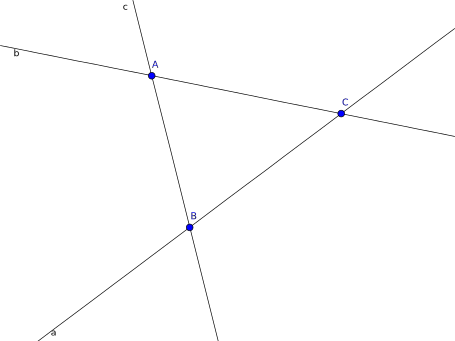
\includegraphics{lec04.files/triangle.svg}
\caption{triangle}
\end{figure}

{]}

\hypertarget{method-1-corner-based}{%
\subsection{Method 1: Corner-based}\label{method-1-corner-based}}

\begin{itemize}
\tightlist
\item
  Calculate all the areas of triangles with different \emph{corners}.
\item
  Problems:

  \begin{itemize}
  \tightlist
  \item
    In practical applications, there may be many corners.
  \item
    What's more, in practical applications, the worst-case scenario may not be at the corners at all.
  \end{itemize}
\end{itemize}

\hypertarget{method-2-monte-carlo}{%
\subsection{Method 2: Monte Carlo}\label{method-2-monte-carlo}}

\begin{itemize}
\tightlist
\item
  Monte-Carlo or Quasi Monte-Carlo:

  \begin{itemize}
  \tightlist
  \item
    Calculate the area of triangles for different sampling points.
  \end{itemize}
\item
  Advantage: more accurate when there are more sampling points.
\item
  Disadvantage: time consuming
\end{itemize}

class: center, middle

\hypertarget{interval-arithmetic-vs.-affine-arithmetic}{%
\section{Interval Arithmetic vs.~Affine Arithmetic}\label{interval-arithmetic-vs.-affine-arithmetic}}

\hypertarget{method-3-interval-arithmetic}{%
\subsection{Method 3: Interval Arithmetic}\label{method-3-interval-arithmetic}}

\begin{itemize}
\tightlist
\item
  Interval arithmetic (IA) estimation:

  \begin{itemize}
  \tightlist
  \item
    Let px = {[}2, 3{]}, py = {[}3, 4{]}
  \item
    Let qx = {[}-5, -4{]}, qy = {[}-6, -5{]}
  \item
    Let rx = {[}6, 7{]} , ry = {[}-5, -4{]}
  \end{itemize}
\item
  Area of triangle:

  \begin{itemize}
  \tightlist
  \item
    = ((qx - px)(ry - py) - (qy - py)(rx - px))/2
  \item
    = {[}33 .. 61{]} (actually {[}36.5 .. 56.5{]})
  \end{itemize}
\item
  Problem: cannot handle \emph{correlation} between variables.
\end{itemize}

\hypertarget{method-4-affine-arithmetic}{%
\subsection{Method 4: Affine Arithmetic}\label{method-4-affine-arithmetic}}

\begin{itemize}
\tightlist
\item
  (Definition to be given shortly)
\item
  More accurate estimation than IA:

  \begin{itemize}
  \tightlist
  \item
    Area = {[}35 .. 57{]} in the previous example.
  \end{itemize}
\item
  Take care of first-order correlation.
\item
  Usually faster than Monte-Carlo, but \ldots.

  \begin{itemize}
  \tightlist
  \item
    becomes inaccurate if the variations are large.
  \end{itemize}
\item
  libaffa.a/YALAA package is publicly available:

  \begin{itemize}
  \tightlist
  \item
    Provides functuins like +, -, *, /, sin(), cos(), pow() etc.
  \end{itemize}
\end{itemize}

\hypertarget{analog-circuit-example}{%
\subsection{Analog Circuit Example}\label{analog-circuit-example}}

\begin{itemize}
\tightlist
\item
  Unit Gain bandwidth

  \begin{itemize}
  \tightlist
  \item
    \texttt{GBW\ =\ sqrt(A*Kp*Ib*(W2/L2)/(2*pi*Cc)} where some parameters are varying
  \end{itemize}
\end{itemize}

\hypertarget{enabling-technologies}{%
\subsection{Enabling Technologies}\label{enabling-technologies}}

\begin{itemize}
\item
  C++ template and operator overloading features greatly simplify the coding effort:
\item
  E.g., the following code can be applied to both \texttt{\textless{}double\textgreater{}} and \texttt{\textless{}AAF\textgreater{}}:

\begin{Shaded}
\begin{Highlighting}[]
\KeywordTok{template}\NormalTok{ \textless{}}\KeywordTok{typename}\NormalTok{ Tp\textgreater{}}
\NormalTok{Tp area(}\AttributeTok{const}\NormalTok{ Tp\& px, }\AttributeTok{const}\NormalTok{ Tp\& qx, }\AttributeTok{const}\NormalTok{ Tp\& rx,}
        \AttributeTok{const}\NormalTok{ Tp\& py, }\AttributeTok{const}\NormalTok{ Tp\& qy, }\AttributeTok{const}\NormalTok{ Tp\& ry) \{}
    \ControlFlowTok{return}\NormalTok{ ((qx{-}px)*(ry{-}py) {-} (qy{-}py)*(rx{-}px)) / }\DecValTok{2}\NormalTok{;}
\NormalTok{\}}
\end{Highlighting}
\end{Shaded}
\item
  In other words, some existing code can be reused with minimal modification.
\end{itemize}

\hypertarget{applications-of-aa}{%
\subsection{Applications of AA}\label{applications-of-aa}}

\begin{itemize}
\tightlist
\item
  Analog Circuit Sizing
\item
  Worst-Case Timing Analysis
\item
  Statistical Static Timing Analysis
\item
  Parameter Variation Interconnect Model Order Reduction {[}CMU02{]}
\item
  Clock Skew Analysis
\item
  Bounded Skew Clock Tree Synthesis
\end{itemize}

\hypertarget{limitations-of-aa}{%
\subsection{Limitations of AA}\label{limitations-of-aa}}

\begin{itemize}
\tightlist
\item
  Something AA can't replace \texttt{\textless{}double\textgreater{}}:

  \begin{itemize}
  \tightlist
  \item
    Iterative methods (no fixed point in AA)
  \item
    No Multiplicative inverse operation (no LU decomposition)
  \item
    Not total ordering, can't sort (???)
  \end{itemize}
\item
  AA can only handle linear correlation, which means you can't expect an accurate approximation of \texttt{abs(x)} near zero.
\item
  Fortunately the ellipsoid method is one of the few algorithms that works with AA.
\end{itemize}

\hypertarget{circuit-sizing-for-op.-amp.}{%
\subsection{Circuit Sizing for Op. Amp.}\label{circuit-sizing-for-op.-amp.}}

\begin{itemize}
\tightlist
\item
  Geometric Programming formulation for CMOS Op. Amp.
\item
  Min-max convex programming under Parametric variations (PVT)
\item
  Ellipsoid Method
\end{itemize}

\hypertarget{what-is-affine-arithmetic}{%
\subsection{What is Affine Arithmetic?}\label{what-is-affine-arithmetic}}

\begin{itemize}
\tightlist
\item
  Represents a quantity x with an affine form (AAF):
  \[\hat{x} = x_0 + x_1 \epsilon_1 + \ldots + x_n \epsilon_n\] where

  \begin{itemize}
  \tightlist
  \item
    noise symbols \(\epsilon_i \in [-1, 1]\)
  \item
    central value \(x_0 \in \mathbb{R}\)
  \item
    partial deviations \(x_i \in \mathbb{R}\)
  \item
    \(n\) is not fixed - new noise symbols are generated during the computation process.
  \end{itemize}
\item
  IA -\textgreater{} AA : \([3..4] \rightarrow 3.5 + 0.5 \epsilon_1\)
\end{itemize}

\hypertarget{geometry-of-aa}{%
\subsection{Geometry of AA}\label{geometry-of-aa}}

.pull-left70{[}

\begin{itemize}
\tightlist
\item
  Affine forms that share noise symbols are dependent:

  \begin{itemize}
  \tightlist
  \item
    \(\hat{x} = x_0 + x_1 \epsilon_1 + \ldots + x_n \epsilon_n\)
  \item
    \(\hat{y} = y_0 + y_1 \epsilon_1 + \ldots + y_m \epsilon_m\)
  \end{itemize}
\item
  The region containing (x, y) is:

  \begin{itemize}
  \tightlist
  \item
    \(Z = \{(x, y) : \epsilon_i \in [-1, 1]\}\)
  \item
    This region is a centrally symmetric convex polygon called ``zonotope''.
  \end{itemize}
\end{itemize}

{]} .pull-right30{[}

\begin{figure}
\centering

\includegraphics{lec04.files/zonotope.svg}
\caption{zonotope}
\end{figure}

{]}

\hypertarget{affine-arithmetic}{%
\subsection{Affine Arithmetic}\label{affine-arithmetic}}

How to find \(\sup_{q \in {\mathbb{Q}}} f_j(x,q)\) efficiently?

\begin{itemize}
\tightlist
\item
  \(\sup_{q \in {\mathbb{Q}}} f_j(x,q)\) is in general difficult to obtain.
\item
  Provided that variations are small or nearly linear, we propose using Affine Arithmetic (AA) to solve this problem.
\item
  Features of AA:

  \begin{itemize}
  \tightlist
  \item
    Handle correlation of variations by sharing \emph{noise symbols}.
  \item
    Enabling technology: template and operator overloading features of C++.
  \item
    A C++ package ``YALAA'' is publicly available.
  \end{itemize}
\end{itemize}

\hypertarget{affine-arithmetic-for-worst-case-analysis}{%
\subsection{Affine Arithmetic for Worst Case Analysis}\label{affine-arithmetic-for-worst-case-analysis}}

\begin{itemize}
\tightlist
\item
  An uncertain quantity is represented in an affine form (AAF):
  \[\hat{a} = a_0 + a_1 \varepsilon_1 + a_2 \varepsilon_2 +
    \cdots +  a_k \varepsilon_k = a_0 + \sum_{i=1}^{k} a_i \varepsilon_i,\]
  where

  \begin{itemize}
  \tightlist
  \item
    \(\varepsilon_i \in [-1, 1]\) is called \emph{noise symbol}.
  \end{itemize}
\item
  Exact results for affine operations (\(\hat{a}+\hat{b}\),
  \(\hat{a}-\hat{b}\) and \(\alpha \cdot \hat{a}\))
\item
  Results of non-affine operations (such as \(\hat{a} \cdot \hat{b}\), \(\hat{a}/\hat{b}\), \(\max(\hat{a}, \hat{b}), \log(\hat{a})\)) are \emph{approximated} in an affine form.
\item
  AA has been applied to a wide range of applications recently when process variations are considered.
\end{itemize}

\hypertarget{affine-arithmetic-for-optimization}{%
\subsection{Affine Arithmetic for Optimization}\label{affine-arithmetic-for-optimization}}

In our robust GP problem:

\begin{itemize}
\tightlist
\item
  First, represent every elements in \(q\) in affine forms.
\item
  For each ellipsoid iteration, \(f(x_c,q)\) is obtained by \emph{approximating} \(f(x_c,\hat{q})\) in an affine form:
  \[\hat{f} = f_0 + f_1 \varepsilon_1 + f_2 \varepsilon_2 + \cdots +  f_k \varepsilon_k.\]
\item
  Then the maximum of \(\hat{f}\) is determined by:
  \[\varepsilon_j = \left\{ \begin{array}{ll}
                +1 & \qquad \text{if} \; f_j > 0 \\
                -1 & \qquad \text{if} \; f_j < 0
              \end{array}
    \right.   \quad j=1, \cdots, k.\]
\end{itemize}

.pull-left70{[}

\begin{figure}
\centering
\includegraphics{lec04.files/pic4.png}
\caption{img}
\end{figure}

{]}

\hypertarget{performance-specification}{%
\subsection{Performance Specification}\label{performance-specification}}

.column-2.font-sm.mb-xs{[}

\begin{longtable}[]{@{}lll@{}}
\toprule
\begin{minipage}[b]{0.35\columnwidth}\raggedright
Constraint\strut
\end{minipage} & \begin{minipage}[b]{0.28\columnwidth}\raggedright
Spec.\strut
\end{minipage} & \begin{minipage}[b]{0.28\columnwidth}\raggedright
Units\strut
\end{minipage}\tabularnewline
\midrule
\endhead
\begin{minipage}[t]{0.35\columnwidth}\raggedright
Device Width\strut
\end{minipage} & \begin{minipage}[t]{0.28\columnwidth}\raggedright
\(\geq 2.0\)\strut
\end{minipage} & \begin{minipage}[t]{0.28\columnwidth}\raggedright
\(\mu\)m\strut
\end{minipage}\tabularnewline
\begin{minipage}[t]{0.35\columnwidth}\raggedright
Device Length\strut
\end{minipage} & \begin{minipage}[t]{0.28\columnwidth}\raggedright
\(\geq 1.0\)\strut
\end{minipage} & \begin{minipage}[t]{0.28\columnwidth}\raggedright
\(\mu\)m\strut
\end{minipage}\tabularnewline
\begin{minipage}[t]{0.35\columnwidth}\raggedright
Estimated Area\strut
\end{minipage} & \begin{minipage}[t]{0.28\columnwidth}\raggedright
minimize\strut
\end{minipage} & \begin{minipage}[t]{0.28\columnwidth}\raggedright
\(\mu\)m\(^2\)\strut
\end{minipage}\tabularnewline
\begin{minipage}[t]{0.35\columnwidth}\raggedright
Input CM Voltage\strut
\end{minipage} & \begin{minipage}[t]{0.28\columnwidth}\raggedright
\([0.45,0.55]\)\strut
\end{minipage} & \begin{minipage}[t]{0.28\columnwidth}\raggedright
x \(V_{DD}\)\strut
\end{minipage}\tabularnewline
\begin{minipage}[t]{0.35\columnwidth}\raggedright
Output Range\strut
\end{minipage} & \begin{minipage}[t]{0.28\columnwidth}\raggedright
\([0.1,0.9]\)\strut
\end{minipage} & \begin{minipage}[t]{0.28\columnwidth}\raggedright
x \(V_{DD}\)\strut
\end{minipage}\tabularnewline
\begin{minipage}[t]{0.35\columnwidth}\raggedright
Gain\strut
\end{minipage} & \begin{minipage}[t]{0.28\columnwidth}\raggedright
\(\geq 80\)\strut
\end{minipage} & \begin{minipage}[t]{0.28\columnwidth}\raggedright
dB\strut
\end{minipage}\tabularnewline
\begin{minipage}[t]{0.35\columnwidth}\raggedright
Unity Gain Freq.\strut
\end{minipage} & \begin{minipage}[t]{0.28\columnwidth}\raggedright
\(\geq 50\)\strut
\end{minipage} & \begin{minipage}[t]{0.28\columnwidth}\raggedright
MHz\strut
\end{minipage}\tabularnewline
\begin{minipage}[t]{0.35\columnwidth}\raggedright
Phase Margin\strut
\end{minipage} & \begin{minipage}[t]{0.28\columnwidth}\raggedright
\(\geq 60\)\strut
\end{minipage} & \begin{minipage}[t]{0.28\columnwidth}\raggedright
degree\strut
\end{minipage}\tabularnewline
\begin{minipage}[t]{0.35\columnwidth}\raggedright
Slew Rate\strut
\end{minipage} & \begin{minipage}[t]{0.28\columnwidth}\raggedright
\(\geq 50\)\strut
\end{minipage} & \begin{minipage}[t]{0.28\columnwidth}\raggedright
V/\(\mu\)s\strut
\end{minipage}\tabularnewline
\begin{minipage}[t]{0.35\columnwidth}\raggedright
CMRR\strut
\end{minipage} & \begin{minipage}[t]{0.28\columnwidth}\raggedright
\(\geq 75\)\strut
\end{minipage} & \begin{minipage}[t]{0.28\columnwidth}\raggedright
dB\strut
\end{minipage}\tabularnewline
\begin{minipage}[t]{0.35\columnwidth}\raggedright
Neg. PSRR\strut
\end{minipage} & \begin{minipage}[t]{0.28\columnwidth}\raggedright
\(\geq 80\)\strut
\end{minipage} & \begin{minipage}[t]{0.28\columnwidth}\raggedright
dB\strut
\end{minipage}\tabularnewline
\begin{minipage}[t]{0.35\columnwidth}\raggedright
Power\strut
\end{minipage} & \begin{minipage}[t]{0.28\columnwidth}\raggedright
\(\leq 3\)\strut
\end{minipage} & \begin{minipage}[t]{0.28\columnwidth}\raggedright
mW\strut
\end{minipage}\tabularnewline
\begin{minipage}[t]{0.35\columnwidth}\raggedright
Noise, Flicker\strut
\end{minipage} & \begin{minipage}[t]{0.28\columnwidth}\raggedright
\(\leq 800\)\strut
\end{minipage} & \begin{minipage}[t]{0.28\columnwidth}\raggedright
nV/Hz\(^{0.5}\)\strut
\end{minipage}\tabularnewline
\bottomrule
\end{longtable}

{]}

\hypertarget{open-loop-gain-example}{%
\subsection{Open-Loop Gain (Example)}\label{open-loop-gain-example}}

\begin{itemize}
\item
  Open-loop gain \(A_v\) can be approximated as a monomial function:

  \[A_v =  \frac{2 C_{ox}}{(\lambda_n + \lambda_p)^2} \sqrt{\mu_n \mu_p \frac{W_1 W_6}{L_1 L_6 I_1 I_6}}\]

  where \(I_1\) and \(I_6\) are monomial functions.
\item
  Corresponding C++ code fragment:

\begin{Shaded}
\begin{Highlighting}[]
\CommentTok{// Open Loop Gain}
\NormalTok{monomial\textless{}aaf\textgreater{} OLG = }\DecValTok{2}\NormalTok{*COX/square(LAMBDAN+LAMBDAP)*}
\NormalTok{     sqrt(KP*KN*W[}\DecValTok{1}\NormalTok{]/L[}\DecValTok{1}\NormalTok{]*W[}\DecValTok{6}\NormalTok{]/L[}\DecValTok{6}\NormalTok{]/I1/I6);}
\end{Highlighting}
\end{Shaded}
\end{itemize}

\hypertarget{results-of-design-variables}{%
\subsection{Results of Design Variables}\label{results-of-design-variables}}

.column-2.font-sm.mb-xs{[}

\begin{longtable}[]{@{}lllll@{}}
\toprule
\begin{minipage}[b]{0.25\columnwidth}\raggedright
Variable\strut
\end{minipage} & \begin{minipage}[b]{0.15\columnwidth}\raggedright
Units\strut
\end{minipage} & \begin{minipage}[b]{0.18\columnwidth}\raggedright
GGPLAB\strut
\end{minipage} & \begin{minipage}[b]{0.13\columnwidth}\raggedright
Our\strut
\end{minipage} & \begin{minipage}[b]{0.15\columnwidth}\raggedright
Robust\strut
\end{minipage}\tabularnewline
\midrule
\endhead
\begin{minipage}[t]{0.25\columnwidth}\raggedright
\(W_1\)\strut
\end{minipage} & \begin{minipage}[t]{0.15\columnwidth}\raggedright
\(\mu\)m\strut
\end{minipage} & \begin{minipage}[t]{0.18\columnwidth}\raggedright
44.8\strut
\end{minipage} & \begin{minipage}[t]{0.13\columnwidth}\raggedright
44.9\strut
\end{minipage} & \begin{minipage}[t]{0.15\columnwidth}\raggedright
45.4\strut
\end{minipage}\tabularnewline
\begin{minipage}[t]{0.25\columnwidth}\raggedright
\(W_8\)\strut
\end{minipage} & \begin{minipage}[t]{0.15\columnwidth}\raggedright
\(\mu\)m\strut
\end{minipage} & \begin{minipage}[t]{0.18\columnwidth}\raggedright
3.94\strut
\end{minipage} & \begin{minipage}[t]{0.13\columnwidth}\raggedright
3.98\strut
\end{minipage} & \begin{minipage}[t]{0.15\columnwidth}\raggedright
3.8\strut
\end{minipage}\tabularnewline
\begin{minipage}[t]{0.25\columnwidth}\raggedright
\(W_{10}\)\strut
\end{minipage} & \begin{minipage}[t]{0.15\columnwidth}\raggedright
\(\mu\)m\strut
\end{minipage} & \begin{minipage}[t]{0.18\columnwidth}\raggedright
2.0\strut
\end{minipage} & \begin{minipage}[t]{0.13\columnwidth}\raggedright
2.0\strut
\end{minipage} & \begin{minipage}[t]{0.15\columnwidth}\raggedright
2.0\strut
\end{minipage}\tabularnewline
\begin{minipage}[t]{0.25\columnwidth}\raggedright
\(W_{13}\)\strut
\end{minipage} & \begin{minipage}[t]{0.15\columnwidth}\raggedright
\(\mu\)m\strut
\end{minipage} & \begin{minipage}[t]{0.18\columnwidth}\raggedright
2.0\strut
\end{minipage} & \begin{minipage}[t]{0.13\columnwidth}\raggedright
2.0\strut
\end{minipage} & \begin{minipage}[t]{0.15\columnwidth}\raggedright
2.1\strut
\end{minipage}\tabularnewline
\begin{minipage}[t]{0.25\columnwidth}\raggedright
\(L_1\)\strut
\end{minipage} & \begin{minipage}[t]{0.15\columnwidth}\raggedright
\(\mu\)m\strut
\end{minipage} & \begin{minipage}[t]{0.18\columnwidth}\raggedright
1.0\strut
\end{minipage} & \begin{minipage}[t]{0.13\columnwidth}\raggedright
1.0\strut
\end{minipage} & \begin{minipage}[t]{0.15\columnwidth}\raggedright
1.0\strut
\end{minipage}\tabularnewline
\begin{minipage}[t]{0.25\columnwidth}\raggedright
\(L_8\)\strut
\end{minipage} & \begin{minipage}[t]{0.15\columnwidth}\raggedright
\(\mu\)m\strut
\end{minipage} & \begin{minipage}[t]{0.18\columnwidth}\raggedright
1.0\strut
\end{minipage} & \begin{minipage}[t]{0.13\columnwidth}\raggedright
1.0\strut
\end{minipage} & \begin{minipage}[t]{0.15\columnwidth}\raggedright
1.0\strut
\end{minipage}\tabularnewline
\begin{minipage}[t]{0.25\columnwidth}\raggedright
\(L_{10}\)\strut
\end{minipage} & \begin{minipage}[t]{0.15\columnwidth}\raggedright
\(\mu\)m\strut
\end{minipage} & \begin{minipage}[t]{0.18\columnwidth}\raggedright
1.0\strut
\end{minipage} & \begin{minipage}[t]{0.13\columnwidth}\raggedright
1.0\strut
\end{minipage} & \begin{minipage}[t]{0.15\columnwidth}\raggedright
1.0\strut
\end{minipage}\tabularnewline
\begin{minipage}[t]{0.25\columnwidth}\raggedright
\(L_{13}\)\strut
\end{minipage} & \begin{minipage}[t]{0.15\columnwidth}\raggedright
\(\mu\)m\strut
\end{minipage} & \begin{minipage}[t]{0.18\columnwidth}\raggedright
1.0\strut
\end{minipage} & \begin{minipage}[t]{0.13\columnwidth}\raggedright
1.0\strut
\end{minipage} & \begin{minipage}[t]{0.15\columnwidth}\raggedright
1.0\strut
\end{minipage}\tabularnewline
\begin{minipage}[t]{0.25\columnwidth}\raggedright
\(A\)\strut
\end{minipage} & \begin{minipage}[t]{0.15\columnwidth}\raggedright
N/A\strut
\end{minipage} & \begin{minipage}[t]{0.18\columnwidth}\raggedright
10.4\strut
\end{minipage} & \begin{minipage}[t]{0.13\columnwidth}\raggedright
10.3\strut
\end{minipage} & \begin{minipage}[t]{0.15\columnwidth}\raggedright
12.0\strut
\end{minipage}\tabularnewline
\begin{minipage}[t]{0.25\columnwidth}\raggedright
\(B\)\strut
\end{minipage} & \begin{minipage}[t]{0.15\columnwidth}\raggedright
N/A\strut
\end{minipage} & \begin{minipage}[t]{0.18\columnwidth}\raggedright
61.9\strut
\end{minipage} & \begin{minipage}[t]{0.13\columnwidth}\raggedright
61.3\strut
\end{minipage} & \begin{minipage}[t]{0.15\columnwidth}\raggedright
69.1\strut
\end{minipage}\tabularnewline
\begin{minipage}[t]{0.25\columnwidth}\raggedright
\(C_c\)\strut
\end{minipage} & \begin{minipage}[t]{0.15\columnwidth}\raggedright
pF\strut
\end{minipage} & \begin{minipage}[t]{0.18\columnwidth}\raggedright
1.0\strut
\end{minipage} & \begin{minipage}[t]{0.13\columnwidth}\raggedright
1.0\strut
\end{minipage} & \begin{minipage}[t]{0.15\columnwidth}\raggedright
1.0\strut
\end{minipage}\tabularnewline
\begin{minipage}[t]{0.25\columnwidth}\raggedright
\(I_{bias}\)\strut
\end{minipage} & \begin{minipage}[t]{0.15\columnwidth}\raggedright
\(\mu\)A\strut
\end{minipage} & \begin{minipage}[t]{0.18\columnwidth}\raggedright
6.12\strut
\end{minipage} & \begin{minipage}[t]{0.13\columnwidth}\raggedright
6.19\strut
\end{minipage} & \begin{minipage}[t]{0.15\columnwidth}\raggedright
5.54\strut
\end{minipage}\tabularnewline
\bottomrule
\end{longtable}

{]}

\hypertarget{performances}{%
\subsection{Performances}\label{performances}}

.font-sm.mb-xs{[}

\begin{longtable}[]{@{}llll@{}}
\toprule
\begin{minipage}[b]{0.40\columnwidth}\raggedright
Performance (units)\strut
\end{minipage} & \begin{minipage}[b]{0.16\columnwidth}\raggedright
Spec.\strut
\end{minipage} & \begin{minipage}[b]{0.16\columnwidth}\raggedright
Std.\strut
\end{minipage} & \begin{minipage}[b]{0.16\columnwidth}\raggedright
Robust\strut
\end{minipage}\tabularnewline
\midrule
\endhead
\begin{minipage}[t]{0.40\columnwidth}\raggedright
Estimated Area (\(\mu\)m\(^2\))\strut
\end{minipage} & \begin{minipage}[t]{0.16\columnwidth}\raggedright
minimize\strut
\end{minipage} & \begin{minipage}[t]{0.16\columnwidth}\raggedright
5678.4\strut
\end{minipage} & \begin{minipage}[t]{0.16\columnwidth}\raggedright
6119.2\strut
\end{minipage}\tabularnewline
\begin{minipage}[t]{0.40\columnwidth}\raggedright
Output Range (x \(V_{DD}\))\strut
\end{minipage} & \begin{minipage}[t]{0.16\columnwidth}\raggedright
{[}0.1, 0.9{]}\strut
\end{minipage} & \begin{minipage}[t]{0.16\columnwidth}\raggedright
{[}0.07, 0.92{]}\strut
\end{minipage} & \begin{minipage}[t]{0.16\columnwidth}\raggedright
{[}0.07, 0.92{]}\strut
\end{minipage}\tabularnewline
\begin{minipage}[t]{0.40\columnwidth}\raggedright
Comm Inp Range (x \(V_{DD}\))\strut
\end{minipage} & \begin{minipage}[t]{0.16\columnwidth}\raggedright
{[}0.45, 0.55{]}\strut
\end{minipage} & \begin{minipage}[t]{0.16\columnwidth}\raggedright
{[}0.41, 0.59{]}\strut
\end{minipage} & \begin{minipage}[t]{0.16\columnwidth}\raggedright
{[}0.39, 0.61{]}\strut
\end{minipage}\tabularnewline
\begin{minipage}[t]{0.40\columnwidth}\raggedright
Gain (dB)\strut
\end{minipage} & \begin{minipage}[t]{0.16\columnwidth}\raggedright
\(\geq 80\)\strut
\end{minipage} & \begin{minipage}[t]{0.16\columnwidth}\raggedright
80\strut
\end{minipage} & \begin{minipage}[t]{0.16\columnwidth}\raggedright
{[}80.0, 81.1{]}\strut
\end{minipage}\tabularnewline
\begin{minipage}[t]{0.40\columnwidth}\raggedright
Unity Gain Freq. (MHz)\strut
\end{minipage} & \begin{minipage}[t]{0.16\columnwidth}\raggedright
\(\geq 50\)\strut
\end{minipage} & \begin{minipage}[t]{0.16\columnwidth}\raggedright
50\strut
\end{minipage} & \begin{minipage}[t]{0.16\columnwidth}\raggedright
{[}50.0, 53.1{]}\strut
\end{minipage}\tabularnewline
\begin{minipage}[t]{0.40\columnwidth}\raggedright
Phase Margin (degree)\strut
\end{minipage} & \begin{minipage}[t]{0.16\columnwidth}\raggedright
\(\geq 60\)\strut
\end{minipage} & \begin{minipage}[t]{0.16\columnwidth}\raggedright
86.5\strut
\end{minipage} & \begin{minipage}[t]{0.16\columnwidth}\raggedright
{[}86.1, 86.6{]}\strut
\end{minipage}\tabularnewline
\begin{minipage}[t]{0.40\columnwidth}\raggedright
Slew Rate (V/\(\mu\)s)\strut
\end{minipage} & \begin{minipage}[t]{0.16\columnwidth}\raggedright
\(\geq 50\)\strut
\end{minipage} & \begin{minipage}[t]{0.16\columnwidth}\raggedright
64\strut
\end{minipage} & \begin{minipage}[t]{0.16\columnwidth}\raggedright
{[}66.7, 66.7{]}\strut
\end{minipage}\tabularnewline
\begin{minipage}[t]{0.40\columnwidth}\raggedright
CMRR (dB)\strut
\end{minipage} & \begin{minipage}[t]{0.16\columnwidth}\raggedright
\(\geq 75\)\strut
\end{minipage} & \begin{minipage}[t]{0.16\columnwidth}\raggedright
77.5\strut
\end{minipage} & \begin{minipage}[t]{0.16\columnwidth}\raggedright
{[}77.5, 78.6{]}\strut
\end{minipage}\tabularnewline
\begin{minipage}[t]{0.40\columnwidth}\raggedright
Neg. PSRR (dB)\strut
\end{minipage} & \begin{minipage}[t]{0.16\columnwidth}\raggedright
\(\geq 80\)\strut
\end{minipage} & \begin{minipage}[t]{0.16\columnwidth}\raggedright
83.5\strut
\end{minipage} & \begin{minipage}[t]{0.16\columnwidth}\raggedright
{[}83.5, 84.6{]}\strut
\end{minipage}\tabularnewline
\begin{minipage}[t]{0.40\columnwidth}\raggedright
Power (mW)\strut
\end{minipage} & \begin{minipage}[t]{0.16\columnwidth}\raggedright
\(\leq 3\)\strut
\end{minipage} & \begin{minipage}[t]{0.16\columnwidth}\raggedright
1.5\strut
\end{minipage} & \begin{minipage}[t]{0.16\columnwidth}\raggedright
{[}1.5, 1.5{]}\strut
\end{minipage}\tabularnewline
\begin{minipage}[t]{0.40\columnwidth}\raggedright
Noise, Flicker (nV/Hz\(^{0.5}\))\strut
\end{minipage} & \begin{minipage}[t]{0.16\columnwidth}\raggedright
\(\leq 800\)\strut
\end{minipage} & \begin{minipage}[t]{0.16\columnwidth}\raggedright
\(600\)\strut
\end{minipage} & \begin{minipage}[t]{0.16\columnwidth}\raggedright
{[}578, 616{]}\strut
\end{minipage}\tabularnewline
\bottomrule
\end{longtable}

{]}

\hypertarget{conclusions}{%
\subsection{Conclusions}\label{conclusions}}

\begin{itemize}
\tightlist
\item
  Our ellipsoid method is fast enough for practical analog circuit
  sizing (take \textless{} 1 sec.~running on a 3GHz Intel CPU for our example).
\item
  Our method is reliable, in the sense that the solution, once
  produced, always satisfies the specification requirement in the
  worst case.
\end{itemize}

\hypertarget{comments}{%
\subsection{Comments}\label{comments}}

\begin{itemize}
\tightlist
\item
  The marriage of AA (algebra) and Zonotope (geometry) has the potential to provide us with a powerful tool for algorithm design.
\item
  AA does not solve all problems. E.g. Iterative method does not apply to AA because AA is not in the Banach space (the fixed-point theorem does not hold).
\item
  AA * and + do not obey the laws of distribution (c.f. floating-point arithmetic)
\item
  AA can only perform first-order approximations. In other words, it can only be applied to nearly linear variations.
\item
  In practice, we still need to combine AA with other methods, such as statistical method or the (quasi-) Monte Carlo method.
\end{itemize}

\end{document}
